\documentclass[11pt,a4paper,oneside]{report}

% --- Packages ---
\usepackage[utf8]{inputenc}
\usepackage[T1]{fontenc}
\usepackage{ae,aecompl,amsfonts}
\usepackage{amsmath,amssymb}
\usepackage[margin=1in]{geometry}
\usepackage{xcolor}
\usepackage{graphicx}
\usepackage{booktabs}
\usepackage{tcolorbox}
\tcbuselibrary{skins,breakable}
\usepackage{tikz}
\usetikzlibrary{arrows.meta, positioning, shapes.geometric, backgrounds, fit}
\usepackage{pgfplots}
\pgfplotsset{compat=1.17}
\usepackage{listings}
\usepackage[colorlinks=true, linkcolor=blue!80!black, urlcolor=blue!80!black, citecolor=blue!80!black]{hyperref}
\usepackage{fancyhdr}
\usepackage{titlesec}
\usepackage{longtable}
\usepackage{colortbl}

% --- Color Palette ---
\definecolor{primaryDark}{RGB}{15, 23, 42}       % Slate 900
\definecolor{primaryBlue}{RGB}{2, 132, 199}      % Sky 600
\definecolor{accentGreen}{RGB}{16, 185, 129}     % Emerald 500
\definecolor{accentAmber}{RGB}{245, 158, 11}     % Amber 500
\definecolor{accentRed}{RGB}{239, 68, 68}        % Red 500
\definecolor{bgGray}{RGB}{248, 250, 252}         % Slate 50
\definecolor{cardBorder}{RGB}{226, 232, 240}     % Slate 200

% --- Listings Settings ---
\lstdefinelanguage{json}{
    basicstyle=\ttfamily\small\color{primaryDark},
    string=[s]{"}{"},
    stringstyle=\color{accentGreen!80!black},
    commentstyle=\color{gray},
    numbers=left,
    numberstyle=\tiny\color{gray},
    numbersep=8pt,
    stepnumber=1,
    breaklines=true,
    frame=single,
    rulecolor=\color{cardBorder}
}

\lstset{
    backgroundcolor=\color{bgGray},
    basicstyle=\ttfamily\small\color{primaryDark},
    keywordstyle=\bfseries\color{primaryBlue},
    commentstyle=\itshape\color{gray},
    stringstyle=\color{accentGreen!80!black},
    numbers=left,
    numberstyle=\tiny\color{gray},
    numbersep=8pt,
    stepnumber=1,
    breaklines=true,
    breakatwhitespace=true,
    frame=single,
    rulecolor=\color{cardBorder},
    tabsize=2,
    showspaces=false,
    showstringspaces=false
}

% --- Custom TColorBox Styles ---
\tcbset{
    storybox/.style={
        colback=primaryBlue!5,
        colframe=primaryBlue,
        coltitle=white,
        fonttitle=\bfseries\sffamily,
        sharp corners,
        rounded corners=southeast,
        arc=3mm,
        boxrule=1.5pt,
        left=12pt,
        right=12pt,
        top=10pt,
        bottom=10pt
    },
    technicalbox/.style={
        colback=bgGray,
        colframe=primaryDark,
        coltitle=white,
        fonttitle=\bfseries\sffamily,
        sharp corners,
        boxrule=1.5pt,
        left=12pt,
        right=12pt,
        top=10pt,
        bottom=10pt
    },
    summarybox/.style={
        colback=accentGreen!5,
        colframe=accentGreen,
        coltitle=white,
        fonttitle=\bfseries\sffamily,
        sharp corners,
        rounded corners=southwest,
        arc=3mm,
        boxrule=1.5pt,
        left=12pt,
        right=12pt,
        top=10pt,
        bottom=10pt
    }
}

% --- Header & Footer ---
\pagestyle{fancy}
\fancyhf{}
\fancyhead[L]{\sffamily\small Quizard Features Storybook: Master Technical Guide}
\fancyhead[R]{\sffamily\small\thepage}
\fancyfoot[C]{\sffamily\footnotesize Confidential --- Digital For Good Engineering Documentation}
\renewcommand{\headrulewidth}{0.6pt}
\renewcommand{\footrulewidth}{0.6pt}

% --- Chapter & Section Formatting ---
\titleformat{\chapter}[display]
  {\normalfont\sffamily\huge\bfseries\color{primaryDark}}{\chaptertitlename\ \thechapter}{15pt}{\Huge}
\titleformat{\section}
  {\normalfont\sffamily\Large\bfseries\color{primaryBlue}}{\thesection}{1em}{}
\titleformat{\subsection}
  {\normalfont\sffamily\large\bfseries\color{primaryDark}}{\thesubsection}{1em}{}

\begin{document}

% --- Title Page ---
\begin{titlepage}
    \centering
    \vspace*{1.5cm}
    
    {\Huge\bfseries\sffamily\color{primaryDark} QUIZARD FEATURES STORYBOOK}\\[0.4cm]
    {\LARGE\bfseries\sffamily\color{primaryBlue} Master Architecture, Gameplay Mechanics, and Tournament Systems}\\[0.8cm]
    
    \rule{\linewidth}{1.5pt}\\[1.0cm]
    
    \begin{tcolorbox}[colback=primaryBlue!5,colframe=primaryBlue,width=0.95\linewidth,arc=2mm]
        \centering
        \large\sffamily
        A Comprehensive Technical Specification and Narrative Guide for Decision Makers, Product Managers, and Backend Software Engineers
    \end{tcolorbox}
    
    \vspace{1.5cm}
    
    \begin{tcolorbox}[colback=white,colframe=cardBorder,width=0.95\linewidth,arc=2mm,title=\textbf{\sffamily Core System Pillars Covered}]
        \begin{itemize}\small
            \item \textbf{Dynamic Rules Governance:} Server-driven timers (180s), 60-question sets, and 2-attempt daily limits
            \item \textbf{High-Speed Question Engine:} Sub-50ms ID sampling, difficulty weighting, and anti-memorization exclusions
            \item \textbf{Military-Grade Cryptography:} AES-256-CBC payload encryption and anti-cheat answering velocity verification
            \item \textbf{Live Leaderboards \& Tie-Breaking:} Real-time SQL window ranking and strict time-based tie resolution
            \item \textbf{Automated Tournament Crons:} 04:30 AM daily billing verification and Thursday 05:30 AM weekly championships
            \item \textbf{Clean Architecture Migration:} Transitioning from Django REST to high-throughput .NET 10 on PostgreSQL
            \item \textbf{High-Velocity Telemetry Gateway:} Dedicated FastAPI microservice (\texttt{cms.quizard.live}) on MongoDB \& Redis
            \item \textbf{CMS Operations \& Telco Billing:} Question approval lifecycles, Wordly, Speed Math, DOB, and bKash passes
            \item \textbf{Financial Reporting \& BI Engine:} Multi-tier winner audits, automated bKash B2C payouts, and revenue analytics
            \item \textbf{Score-Driven Performance Bands:} 6 score-driven tiers (0 to 60) with asymmetric delta adjustments
            \item \textbf{XP Ledger \& Linear Streaks:} Linear daily streak progression ($+20\text{ XP}\times n$) with giant Day 15 milestone surge
            \item \textbf{Rank Velocity \& Adaptive Challenge:} Live $\uparrow/\downarrow$ glyphs, personalized cards, and 10s fast timers
        \end{itemize}
    \end{tcolorbox}
    
    \vfill
    {\bfseries Author:} Engineering Architecture Team\\
    {\bfseries Ecosystem:} Next.js 16 Frontend $\longleftrightarrow$ Quizard-API (FastAPI / MongoDB) $\longleftrightarrow$ .NET 10 (PostgreSQL)\\
    {\bfseries Database Cluster:} PostgreSQL Enterprise Cluster (Host: 103.174.50.155) + MongoDB Telemetry Cluster\\
    {\bfseries Date:} August 2026
\end{titlepage}

% --- Table of Contents ---
\tableofcontents
\newpage

% --- Executive Overview ---
\chapter*{Executive Overview: The Quizard Platform}
\addcontentsline{toc}{chapter}{Executive Overview: The Quizard Platform}

\begin{tcolorbox}[storybox, title={Platform Mission}]
Quizard is Bangladesh's premier real-time interactive quiz and tournament platform, engaging hundreds of thousands of concurrent players across web and telecommunication partner channels (bKash, Banglalink, Robi). 

To ensure absolute competitive integrity, fair prize distribution, and instantaneous responsiveness, Quizard combines server-authoritative game governance, sub-50ms dynamic question generation, end-to-end payload cryptography, and automated tournament consolidation.
\end{tcolorbox}

\section*{The End-to-End System Architecture}
The diagram below illustrates the comprehensive lifecycle of a player's journey through Quizard:

\begin{figure}[htbp]
\centering
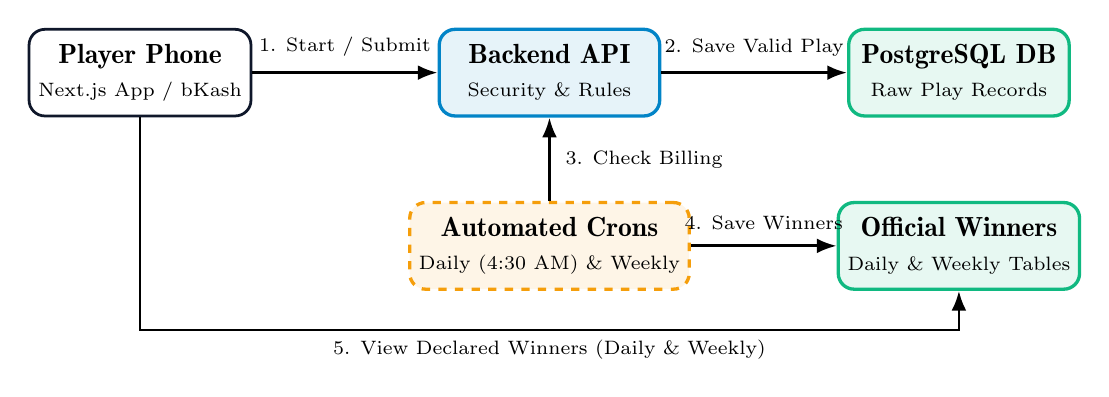
\begin{tikzpicture}[
    node distance=2.2cm,
    box/.style={rectangle, draw=primaryDark, fill=white, rounded corners=2mm, minimum width=2.6cm, minimum height=1.1cm, align=center, line width=1pt},
    apibox/.style={rectangle, draw=primaryBlue, fill=primaryBlue!10, rounded corners=2mm, minimum width=2.8cm, minimum height=1.1cm, align=center, line width=1.2pt},
    dbbox/.style={rectangle, draw=accentGreen, fill=accentGreen!10, rounded corners=2mm, minimum width=2.8cm, minimum height=1.1cm, align=center, line width=1.2pt},
    cronbox/.style={rectangle, draw=accentAmber, fill=accentAmber!10, dashed, rounded corners=2mm, minimum width=2.8cm, minimum height=1.1cm, align=center, line width=1.2pt}
]
    % Nodes
    \node[box] (phone) at (0, 0) {\textbf{Player Phone}\\\scriptsize Next.js App / bKash};
    \node[apibox] (api) at (5.2, 0) {\textbf{Backend API}\\\scriptsize Security \& Rules};
    \node[dbbox] (db) at (10.4, 0) {\textbf{PostgreSQL DB}\\\scriptsize Raw Play Records};

    \node[cronbox] (cron) at (5.2, -2.2) {\textbf{Automated Crons}\\\scriptsize Daily (4:30 AM) \& Weekly};
    \node[dbbox] (winners) at (10.4, -2.2) {\textbf{Official Winners}\\\scriptsize Daily \& Weekly Tables};

    % Arrows
    \draw[-{Latex[length=2.5mm]}, line width=1pt] (phone) -- node[above, yshift=2pt]{\scriptsize 1. Start / Submit} (api);
    \draw[-{Latex[length=2.5mm]}, line width=1pt] (api) -- node[above, yshift=2pt]{\scriptsize 2. Save Valid Play} (db);
    \draw[-{Latex[length=2.5mm]}, line width=1pt] (cron) -- node[right, xshift=2pt]{\scriptsize 3. Check Billing} (api);
    \draw[-{Latex[length=2.5mm]}, line width=1pt] (cron) -- node[above, yshift=2pt]{\scriptsize 4. Save Winners} (winners);
    \draw[-{Latex[length=2.5mm]}, line width=1pt] (phone.south) |- ++(0,-2.7) -| node[pos=0.25, below]{\scriptsize 5. View Declared Winners (Daily \& Weekly)} (winners.south);
\end{tikzpicture}
\caption{Quizard End-to-End Competition and Winner Lifecycle}
\end{figure}

\newpage

% --- Chapters Inclusion ---
\input{chapters/chapter1_rules_engine_governance}
\newpage

\input{chapters/chapter2_gameplay_question_engine}
\newpage

\input{chapters/chapter3_security_anticheat_scoring}
\newpage

\input{chapters/chapter4_leaderboards_tournaments_winners}
\newpage

\input{chapters/chapter5_api_architecture_dotnet_migration}
\newpage

\input{chapters/chapter6_cms_fastapi_telemetry_service}
\newpage

\chapter{The Master Ecosystem: CMS Operations, Multi-Game Engines, and Telco Billing}

\begin{tcolorbox}[storybox, title={The Complete Quizard Ecosystem in Brief}]
Beyond rapid 60-question trivia, Quizard is an enterprise gaming ecosystem. It features a multi-tenant Content Management System (CMS) with question approval lifecycles, role-based admin governance, a multi-game suite (Wordly, Speed Math, Memory Match, Sudoku), direct telco operator billing (bKash, Banglalink, GP, Robi), affiliate campaign attribution, and automated financial prize disbursement.
\end{tcolorbox}

\section{The CMS Question Authoring and Approval Pipeline}
High-quality trivia requires rigorous editorial oversight. Quizard's CMS (\texttt{apps.cms}) provides a multi-stage question authoring pipeline:

\begin{figure}[htbp]
\centering
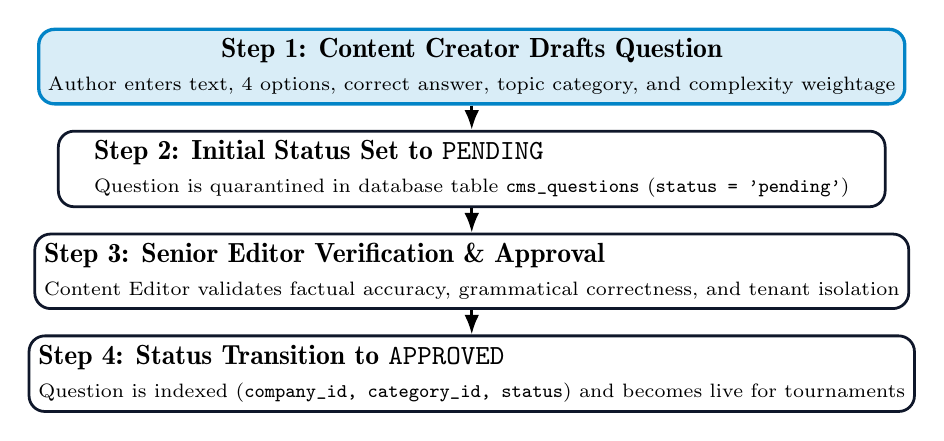
\begin{tikzpicture}[
    node distance=1.3cm,
    stepbox/.style={rectangle, draw=primaryDark, fill=white, rounded corners=2mm, minimum width=10.5cm, minimum height=0.9cm, align=left, line width=1pt},
    headerbox/.style={rectangle, draw=primaryBlue, fill=primaryBlue!15, rounded corners=2mm, minimum width=10.5cm, minimum height=0.9cm, align=center, line width=1.2pt}
]
    \node[headerbox] (h1) at (0, 0) {\textbf{Step 1: Content Creator Drafts Question}\\\scriptsize Author enters text, 4 options, correct answer, topic category, and complexity weightage};
    \node[stepbox] (s2) at (0, -1.3) {\textbf{Step 2: Initial Status Set to \texttt{PENDING}}\\\scriptsize Question is quarantined in database table \texttt{cms\_questions} (\texttt{status = 'pending'})};
    \node[stepbox] (s3) at (0, -2.6) {\textbf{Step 3: Senior Editor Verification \& Approval}\\\scriptsize Content Editor validates factual accuracy, grammatical correctness, and tenant isolation};
    \node[stepbox] (s4) at (0, -3.9) {\textbf{Step 4: Status Transition to \texttt{APPROVED}}\\\scriptsize Question is indexed (\texttt{company\_id, category\_id, status}) and becomes live for tournaments};

    \draw[-{Latex[length=2.5mm]}, line width=1pt] (h1) -- (s2);
    \draw[-{Latex[length=2.5mm]}, line width=1pt] (s2) -- (s3);
    \draw[-{Latex[length=2.5mm]}, line width=1pt] (s3) -- (s4);
\end{tikzpicture}
\caption{The Multi-Stage CMS Question Approval Pipeline}
\end{figure}

\subsection{Data Model of a CMS Question Entity}
Every question entity is strictly bound to its company tenant and topic category:
\begin{lstlisting}[language=python, caption={The Question Entity Data Model}]
class Questions(models.Model):
    company = models.ForeignKey(Company, on_delete=models.CASCADE)
    category = models.ForeignKey(Category, on_delete=models.CASCADE)
    weightage = models.JSONField(default=list) # Difficulty 1 to 6
    question = models.CharField(max_length=400)
    options_nub = models.IntegerField(default=4)
    option1 = models.CharField(max_length=200)
    option2 = models.CharField(max_length=200)
    option3 = models.CharField(max_length=200, null=True, blank=True)
    option4 = models.CharField(max_length=200, null=True, blank=True)
    ans = models.CharField(max_length=200) # e.g. "Option1"
    status = models.CharField(choices=APPROVE_STATUS, default='approved')
\end{lstlisting}

\section{Admin Governance and Role-Based Access Control (RBAC)}
Quizard enforces strict enterprise security using granular Role-Based Access Control (\texttt{apps.cms\_users}):

\begin{itemize}
    \item \textbf{Super Administrator:} Full access across all portals, database settings, financial payout configurations, and user management.
    \item \textbf{Content Manager / Creator:} Restricted to drafting, categorizing, and editing trivia questions within assigned company portals (e.g., Portal 15 bKash vs. Portal 20 Banglalink).
    \item \textbf{Finance \& Operations Auditor:} Read and export access to prize disbursement records (\texttt{apps.disbursmentReport}), daily charging graphs, and bKash payout reconciliation.
    \item \textbf{Partner Admin (Tenant Isolation):} Restricted views allowing telecom partners (Robi, Banglalink) to inspect only their active subscriber counts and tournament leaderboards.
\end{itemize}

\section{The Multi-Game Suite: Beyond Rapid Trivia}
Quizard is a multi-genre gaming platform offering diverse casual and competitive titles:

\subsection{1. Wordly: The Daily Bengali \& English Word Puzzle}
In \texttt{apps.word}, players solve daily 3, 4, 5, and 6-letter word puzzles in both Bengali and English. 
\begin{itemize}
    \item Players have 6 attempts to guess the hidden dictionary word.
    \item Guess telemetry is tracked daily.
    \item Stored procedures \texttt{WordlyWinner} and \texttt{WordlyWeeklyWinner} calculate daily accuracy streaks and award cash prizes to top word puzzle masters.
\end{itemize}

\subsection{2. Speed Math and Addition Sprint}
In \texttt{api/addition}, contestants solve rapid arithmetic challenges against an accelerating timer, testing reflex calculation speed.

\subsection{3. Memory Match and Sudoku Challenges}
In \texttt{api/participants}, puzzle enthusiasts compete in card-matching memory tests and tiered Sudoku difficulties (Foundational, Intermediate, Grandmaster).

\section{Direct Operator Billing (DOB) and Telco Subscriptions}
To monetize games across Bangladesh, Quizard integrates directly with Mobile Network Operators (MNOs) and Mobile Financial Services (MFS):

\begin{figure}[htbp]
\centering
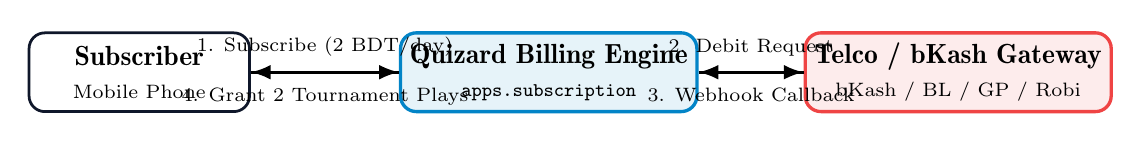
\begin{tikzpicture}[
    node distance=2.0cm,
    box/.style={rectangle, draw=primaryDark, fill=white, rounded corners=2mm, minimum width=2.8cm, minimum height=1.0cm, align=center, line width=1pt},
    apibox/.style={rectangle, draw=primaryBlue, fill=primaryBlue!10, rounded corners=2mm, minimum width=3.0cm, minimum height=1.0cm, align=center, line width=1.2pt},
    mfsbox/.style={rectangle, draw=accentRed, fill=accentRed!10, rounded corners=2mm, minimum width=3.0cm, minimum height=1.0cm, align=center, line width=1.2pt}
]
    \node[box] (user) at (0, 0) {\textbf{Subscriber}\\\scriptsize Mobile Phone};
    \node[apibox] (quizard) at (5.2, 0) {\textbf{Quizard Billing Engine}\\\scriptsize \texttt{apps.subscription}};
    \node[mfsbox] (telco) at (10.4, 0) {\textbf{Telco / bKash Gateway}\\\scriptsize bKash / BL / GP / Robi};

    \draw[-{Latex[length=2.5mm]}, line width=1pt] (user) -- node[above, yshift=2pt]{\scriptsize 1. Subscribe (2 BDT/day)} (quizard);
    \draw[-{Latex[length=2.5mm]}, line width=1pt] (quizard) -- node[above, yshift=2pt]{\scriptsize 2. Debit Request} (telco);
    \draw[-{Latex[length=2.5mm]}, line width=1pt, dashed] (telco) -- node[below, yshift=-2pt]{\scriptsize 3. Webhook Callback} (quizard);
    \draw[-{Latex[length=2.5mm]}, line width=1pt, dashed] (quizard) -- node[below, yshift=-2pt]{\scriptsize 4. Grant 2 Tournament Plays} (user);
\end{tikzpicture}
\caption{Telco Direct Operator Billing (DOB) \& Subscription Lifecycle}
\end{figure}

\begin{itemize}
    \item \textbf{bKash Direct Charging (\texttt{apps.bkash}):} Seamless in-app subscription and one-time tournament passes via tokenized bKash payment APIs.
    \item \textbf{Banglalink Direct Operator Billing (\texttt{apps.banglalink}):} Direct carrier balance deduction with automated renewal crons and unsubscribe postbacks.
    \item \textbf{Grameenphone \& Robi Carrier Integrations (\texttt{apps.grameenphone}, \texttt{apps.webhook}):} High-availability webhook listeners capturing charging successes and subscription renewals.
\end{itemize}

\section{Financial Operations, Referrals, and Prize Disbursements}
Quizard features an automated financial operations suite in \texttt{apps.disbursmentReport}:

\begin{itemize}
    \item \textbf{Micro-Prize Tiers (5 TK \& 10 TK Winners):} Automated stored procedures \texttt{5tkWinner} and \texttt{10tkWinner} aggregate and verify daily runners-up who achieve qualifying scores.
    \item \textbf{Referral Bonus Rewards (\texttt{PrizeOnReferral}, \texttt{ReferHistory}):} When players invite friends using custom referral codes, bonus points and cash bounties are automatically credited upon the referee's first paid tournament round.
    \item \textbf{Automated bKash Payout Gateway:} Once winners are frozen in \texttt{quizapp\_dailywinnerhistorytemp} or \texttt{quizapp\_weeklywinnerhistorytemp}, the finance disbursement engine triggers the bKash Merchant B2C Disbursement API, sending cash directly to the player's bKash wallet.
    \item \textbf{Churn-Back Win-Back Campaigns (\texttt{ChurnBackCashBack}):} Automatically rewards re-activated lapsed subscribers with promotional game passes.
\end{itemize}

\section{Ad Network Attribution and Campaign Tracking}
In \texttt{apps.campaign}, the platform tracks digital marketing acquisition across ad networks:
\begin{itemize}
    \item \textbf{Ad Networks (\texttt{Adnetwork}):} Defines partner ad networks (e.g., Google, Meta, local DSPs), click ID parameters (\texttt{click\_id}), and server-to-server passback postback URLs.
    \item \textbf{Campaigns (\texttt{Campaign}):} Maps promotional campaigns to target portals, automatically converting USD payout rates to BDT ($\text{Payout}_{\text{BDT}} = \text{Payout}_{\text{USD}} \times 120$) and tracking conversion volumes.
\end{itemize}

\section{Real-World Stories: Behind the Scenes}

\subsection{Story 1: Farhana Prepares the National BCS Tournament Questions}
In Dhaka, Farhana is a Senior Content Manager for Quizard. Ahead of the upcoming 46th BCS Preliminary Exam, she uses the CMS admin panel to upload 500 new verified questions across Bangladesh Affairs, International Relations, and General Science.

\begin{enumerate}
    \item She sets category IDs to BCS Prep (\texttt{category = 1}) and complexity weightage from 1 to 5.
    \item The questions are saved as \texttt{status = 'pending'}.
    \item Farhana reviews each question for syllabus accuracy, verifies the 4 options, and approves the batch.
    \item The questions instantly enter the active question pool for tonight's BCS Mega Tournament!
\end{enumerate}

\subsection{Story 2: Rupa Wins the Daily Wordly Challenge in Sylhet}
In Sylhet, Rupa plays the Bengali 5-letter Wordly challenge on \texttt{wordly.quizard.live}. In 4 guesses, she deciphers the hidden 5-letter word \textbf{``POTAKA''} (Flag). 

\begin{enumerate}
    \item Her score and elapsed time are recorded.
    \item At midnight, the \texttt{WordlyWinner} stored procedure runs, verifying her paid bKash subscription and high accuracy.
    \item Rupa wins 500 BDT in prize cash!
\end{enumerate}

\subsection{Story 3: Monir Audits and Disburses Weekly Prizes}
On Thursday at 10:00 AM, Monir, the Operations Finance Lead at Digital For Good, logs into the Disbursement Report portal. 

\begin{enumerate}
    \item He opens \texttt{/report/weeklyWinner.html} to inspect the frozen winners generated by the 05:30 AM weekly cron.
    \item He cross-references subscriber payment counts and clicks ``Approve Payout''.
    \item The bKash B2C disbursement gateway executes, and within seconds, Ayesha in Rajshahi receives an SMS: \textit{``You have received 25,000 BDT from Quizard Tournament!''}
\end{enumerate}

\begin{tcolorbox}[summarybox, title={Chapter Key Takeaways}]
\begin{itemize}
    \item Quizard's CMS guarantees question quality and factual accuracy through a rigorous multi-stage approval workflow.
    \item The platform powers a diverse gaming portfolio including trivia, Wordly word puzzles, speed math, and Sudoku.
    \item Direct carrier billing across bKash, Banglalink, Grameenphone, and Robi ensures seamless monetization across all major telecom networks.
    \item Financial disbursement reports and automated bKash B2C payouts provide transparent, audited, and instant cash prize delivery to verified winners.
\end{itemize}
\end{tcolorbox}

\newpage

\input{chapters/chapter8_reporting_analytics_payouts}
\newpage

\input{chapters/chapter9_rating_algorithm_score_bands}
\newpage

\chapter{The XP Ledger, Linear Daily Streaks, and Milestone Achievement System}

\begin{tcolorbox}[storybox, title={The Retention Gamification Engine in Brief}]
A 15-day live data review revealed that the majority of players churn after a single session. To cultivate enduring daily return habits, Quizard implements an Experience Point (XP) system powered by an immutable transaction ledger, linear daily streak rewards, a giant 15th-day milestone surge, and collectible achievement badges.
\end{tcolorbox}

\section{Core Experience Point (XP) Earning Mechanics}
XP serves as Quizard's primary engagement currency, separate from competitive tournament scores. It is awarded for participation and daily consistency:

\begin{itemize}
    \item \textbf{Daily First-Play Bonus:} $+50\text{ XP}$ awarded on the contestant's first tournament round of the day.
    \item \textbf{Round Completion Base XP:} $+10\text{ XP}$ awarded upon completing each 60-question match.
    \item \textbf{Answer Accuracy Bounty:} $+1\text{ XP}$ per correct answer ($\text{RightCount} \le 60$).
\end{itemize}

\section{Linear Daily Streaks with the Giant 15th-Day Surge}
To foster an intuitive and predictable daily habit loop, the daily streak progression is strictly \textbf{linear}, rewarding each consecutive return day with an incremental boost, culminating in a \textbf{giant milestone bump on the 15th day}.

\subsection{Linear Daily Formula}
For Days 1 through 14:
\begin{equation}
\text{Streak Bonus XP}(\text{Day } n) = 20 \times n
\end{equation}

\subsection{The 15-Day Milestone Progression Matrix}
\begin{table}[htbp]
\centering
\footnotesize
\begin{tabular}{|c|c|p{4.5cm}|p{4.5cm}|}
\hline
\rowcolor{primaryBlue!15}
\textbf{Consecutive Day} & \textbf{Linear Base Bonus} & \textbf{Special Milestone Surge} & \textbf{Total Daily Streak Reward} \\ \hline
\textbf{Day 1} & $+20\text{ XP}$ & -- & $+20\text{ XP}$ \\ \hline
\textbf{Day 2} & $+40\text{ XP}$ & -- & $+40\text{ XP}$ \\ \hline
\textbf{Day 3} & $+60\text{ XP}$ & -- & $+60\text{ XP}$ \\ \hline
\textbf{Day 4} & $+80\text{ XP}$ & -- & $+80\text{ XP}$ \\ \hline
\textbf{Day 5} & $+100\text{ XP}$ & -- & $+100\text{ XP}$ \\ \hline
\textbf{Day 6} & $+120\text{ XP}$ & -- & $+120\text{ XP}$ \\ \hline
\textbf{Day 7} & $+140\text{ XP}$ & Week 1 Streak Badge & $+140\text{ XP} + \text{Bronze Badge}$ \\ \hline
\textbf{Day 8} & $+160\text{ XP}$ & -- & $+160\text{ XP}$ \\ \hline
\textbf{Day 9} & $+180\text{ XP}$ & -- & $+180\text{ XP}$ \\ \hline
\textbf{Day 10} & $+200\text{ XP}$ & -- & $+200\text{ XP}$ \\ \hline
\textbf{Day 11} & $+220\text{ XP}$ & -- & $+220\text{ XP}$ \\ \hline
\textbf{Day 12} & $+240\text{ XP}$ & -- & $+240\text{ XP}$ \\ \hline
\textbf{Day 13} & $+260\text{ XP}$ & -- & $+260\text{ XP}$ \\ \hline
\textbf{Day 14} & $+280\text{ XP}$ & -- & $+280\text{ XP}$ \\ \hline
\rowcolor{accentAmber!20}
\textbf{Day 15} & $+300\text{ XP}$ & \textbf{+2,500 XP Milestone Surge} & $\mathbf{+2,800\text{ \textbf{XP}}} + \text{\textbf{Half-Month Titan}}$ \\ \hline
\textbf{Day 16} & $+320\text{ XP}$ & -- & $+320\text{ XP}$ \\ \hline
\end{tabular}
\caption{Linear Daily Streak Progression with Giant 15th-Day Milestone Bump}
\end{table}

\begin{figure}[htbp]
\centering
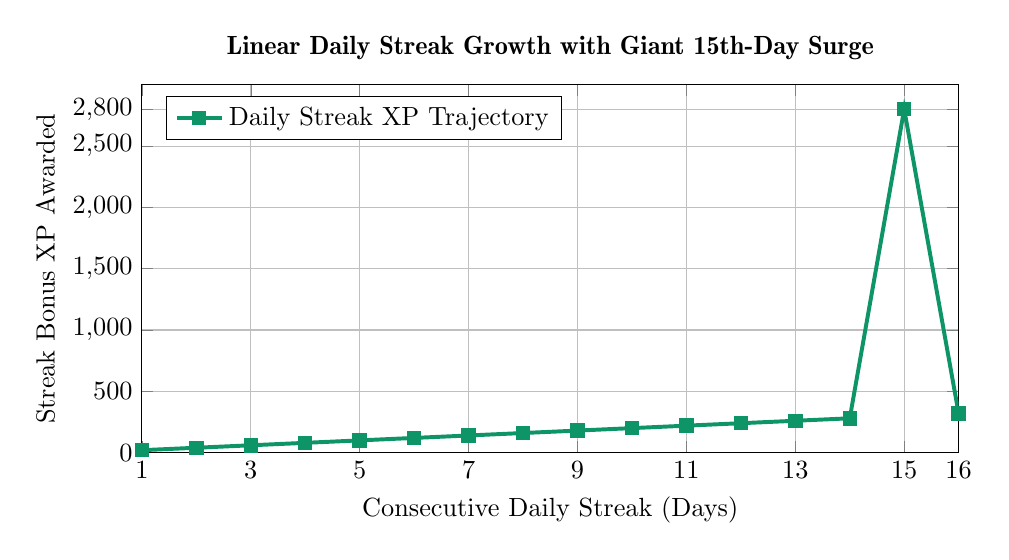
\begin{tikzpicture}[scale=0.95]
    \begin{axis}[
        title={\textbf{Linear Daily Streak Growth with Giant 15th-Day Surge}},
        xlabel={Consecutive Daily Streak (Days)},
        ylabel={Streak Bonus XP Awarded},
        xmin=1, xmax=16,
        ymin=0, ymax=3000,
        xtick={1,3,5,7,9,11,13,15,16},
        ytick={0, 500, 1000, 1500, 2000, 2500, 2800},
        grid=major,
        width=12.5cm, height=6.5cm,
        legend pos=north west
    ]
    \addplot[color=accentGreen!80!black, mark=square*, line width=1.5pt] coordinates {
        (1, 20)
        (2, 40)
        (3, 60)
        (4, 80)
        (5, 100)
        (6, 120)
        (7, 140)
        (8, 160)
        (9, 180)
        (10, 200)
        (11, 220)
        (12, 240)
        (13, 260)
        (14, 280)
        (15, 2800)
        (16, 320)
    };
    \legend{Daily Streak XP Trajectory}
    \end{axis}
\end{tikzpicture}
\caption{Visual Trajectory of Daily Streak Rewards Illustrating the Day 15 Giant Bump}
\end{figure}

\section{Milestone Achievement Badges Shelf}
Contestants unlock permanent collectible badges displayed on their public profiles:

\begin{table}[htbp]
\centering
\small
\begin{tabular}{|l|l|p{6.8cm}|}
\hline
\rowcolor{primaryBlue!15}
\textbf{Badge Name} & \textbf{Tier} & \textbf{Unlock Criteria} \\ \hline
\textbf{First Blood} & Bronze & Win 1st tournament match or place in the daily top 100. \\ \hline
\textbf{Week 1 Champion} & Bronze & Maintain an unbroken 7-day daily gameplay streak. \\ \hline
\textbf{Speed Demon} & Silver & Complete a 60-question round with $\ge 50$ correct in $< 90$ seconds. \\ \hline
\textbf{Quiz Scholar} & Gold & Play all 4 official games (Daily, Sports, BCS, Tournament) in 7 days. \\ \hline
\textbf{Century Club} & Gold & Accumulate 100 total completed tournament rounds. \\ \hline
\textbf{Half-Month Titan}& Platinum & Complete the 15-day unbroken daily streak and claim the giant surge. \\ \hline
\textbf{Master Strategist}& Diamond & Achieve and maintain a rolling score band in \textbf{Master} ($50-59$). \\ \hline
\textbf{Grandmaster Elite}& Diamond & Score a perfect 60/60 in a live tournament championship. \\ \hline
\end{tabular}
\caption{Quizard Milestone Achievement Badges Matrix}
\end{table}

\section{Database Schema and API Architecture}

\subsection{1. PostgreSQL Immutable XP Ledger Table}
\begin{lstlisting}[language=SQL, caption={PostgreSQL Schema for XP Ledger}]
CREATE TABLE participant_xp_ledger (
    id BIGSERIAL PRIMARY KEY,
    msisdn VARCHAR(15) NOT NULL,
    portal_id INT NOT NULL DEFAULT 15,
    xp_amount INT NOT NULL,
    source_event VARCHAR(50) NOT NULL, -- 'daily_login', 'streak_linear', 'streak_day_15_giant_bump', 'quiz_round'
    balance_after INT NOT NULL,
    created_at TIMESTAMP WITH TIME ZONE DEFAULT CURRENT_TIMESTAMP
);
CREATE INDEX idx_xp_ledger_lookup ON participant_xp_ledger (msisdn, portal_id, created_at DESC);
\end{lstlisting}

\subsection{2. REST Endpoints Specification}
\begin{table}[htbp]
\centering
\small
\begin{tabular}{|p{6.2cm}|c|p{7.5cm}|}
\hline
\rowcolor{primaryBlue!15}
\textbf{Endpoint} & \textbf{Method} & \textbf{Payload / Response Description} \\ \hline
\texttt{/api/participantProfile/}\newline\texttt{xp\_summary/} & \texttt{GET} & Returns cumulative XP, current unbroken streak count, and unlocked badge objects. \\ \hline
\end{tabular}
\caption{XP Summary REST Endpoint}
\end{table}

\section{Real-World Scenario: Sabina's 15-Day Streak Journey}
In Dhaka, Sabina commits to playing Quizard every morning during her MRT transit:

\begin{enumerate}
    \item \textbf{Days 1--5:} Sabina earns $+20\text{ XP}, +40\text{ XP}, +60\text{ XP}, +80\text{ XP}$, and $+100\text{ XP}$ alongside her daily first-play bonuses.
    \item \textbf{Day 7:} Unlocks the \textbf{Week 1 Champion} bronze badge.
    \item \textbf{Days 8--14:} Her streak climbs linearly ($+160\text{ XP} \to +280\text{ XP}$).
    \item \textbf{Day 15 (The Giant Surge):} Sabina logs in and completes her morning round. The backend triggers the giant 15th-day milestone, crediting $\mathbf{+2,800\text{ XP}}$, elevating her to Player Level 18, and awarding the coveted \textbf{Half-Month Titan} platinum badge.
\end{enumerate}

\begin{tcolorbox}[summarybox, title={Chapter Key Takeaways}]
\begin{itemize}
    \item The linear streak model ($+20\text{ XP} \times \text{day}$) provides clear daily progression.
    \item The giant 15th-day milestone surge ($+2,800\text{ XP}$) delivers a major gratification climax that dramatically curbs mid-month churn.
    \item The immutable XP ledger guarantees auditable, tamper-proof tracking of all gamification rewards.
\end{itemize}
\end{tcolorbox}

\newpage

\input{chapters/chapter11_rank_velocity_personalization_adaptive}
\newpage

% --- Appendix & Summary ---
\chapter{Technical Glossary and Reference Guide}

\section{Glossary of Core Domain Entities}
\begin{description}
    \item[\textbf{MSISDN:}] Mobile Station International Subscriber Directory Number (the player's unique mobile phone number in Bangladesh, e.g., \texttt{01711000001}).
    \item[\textbf{Event / Rule ID:}] Unique numeric identifier for a tournament competition rule set (e.g., \texttt{Event 34 = Daily Rapid Tournament}, \texttt{Event 75 = Mega Weekly Championship}).
    \item[\textbf{Portal ID:}] Tenant identifier providing multi-tenant isolation (e.g., \texttt{15 = Quizard Web / bKash}, \texttt{20 = Banglalink}, \texttt{21 = Robi}).
    \item[\textbf{AES-256-CBC:}] Advanced Encryption Standard with 256-bit key length operating in Cipher Block Chaining mode, securing all client score transmissions.
    \item[\textbf{Dense Rank:}] A database ranking function where identical scores receive identical rank numbers without creating gaps in consecutive rank assignments.
    \item[\textbf{Velocity Check:}] Anti-cheat validation ensuring the rate of answered questions does not exceed human biological reaction thresholds ($\le 1.5\text{ answers/sec}$).
\end{description}

\begin{tcolorbox}[summarybox, title={Final Architecture Conclusion}]
Quizard's architecture represents a gold standard for high-performance, real-time gaming in emerging markets. By coupling dynamic rules governance, sub-50ms question sampling, end-to-end cryptographic integrity, and automated financial verification, the platform delivers an engaging and trustworthy experience to millions of contestants.
\end{tcolorbox}

\end{document}
